\section{Theorie}
\label{sec:Theorie}

\subsection{Energieniveaus der Rubidiumisotope}
Rubidium ist ein Alkalimetall und besitzt somit ein Elektron in der Valenzschale.
Näherungsweise wird Rubidium durch das Wasserstoff-Atommodell beschrieben.
In diesem Experiment wird ein Gasgemisch aus den Rubidiumisotopen $^{87}\text{Rb}$ und $^{85}\text{Rb}$ betrachtet.
Der Spin des Elektrons beträgt $S=1/2$.
Anders als bei dem Elektronspin unterscheidet sich der Kern signifikant von einem Wasserstoffatom und führt zu einer veränderten Aufspaltung der Energieniveaus.
Die Isotope weisen aufgrund der unterschiedlichen Nukleonenanzahl einen unterschiedlichen Kernspin $I$ auf, wobei $I=3/2$ für $^{87}\text{Rb}$ und $I=5/2$ für $^{85}\text{Rb}$ gilt.
\\
Die Aufspaltung der Energieniveaus beider Isotope ist in \autoref{fig:energieniveaus} dargestellt.
\begin{figure}
    \centering
    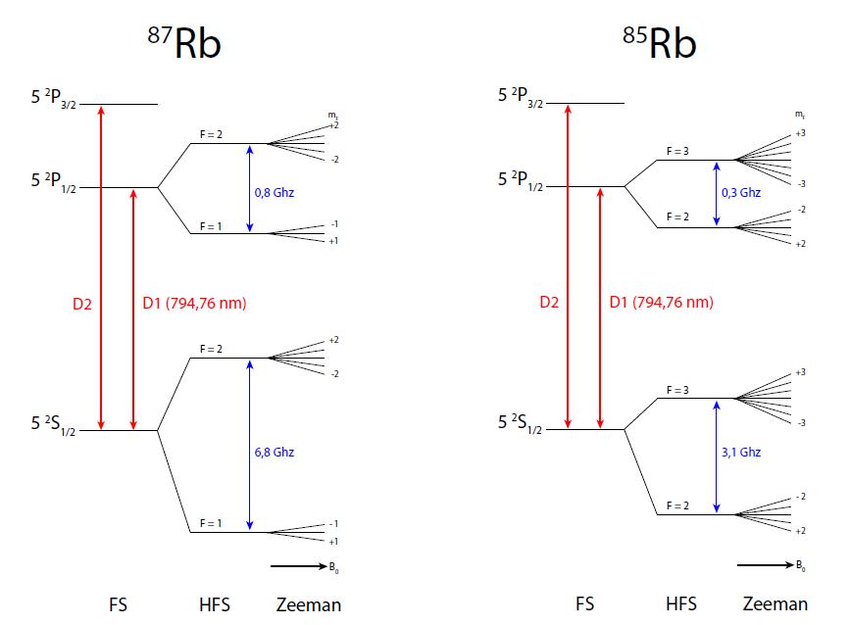
\includegraphics[width=1\textwidth]{content/img/energieniveaus2.png}
    \caption{Schematische Darstellung der Energieniveaus des $^{87}\text{Rb}$- und $^{85}\text{Rb}$-Isotops, 
    wobei die Feinstruktur(\textbf{FS}), die Hyperfeinstruktur(\textbf{HFS}) und die Aufspaltung durch den \textbf{Zeeman}-Effekt betrachtet werden. \cite{borgo}}
    \label{fig:energieniveaus}
\end{figure}
Im folgenden wird die Feinstruktur(\textbf{FS}), die Hyperfeinstruktur(\textbf{HFS}) und die Aufspaltung durch den \textbf{Zeeman}-Effekt der Energieniveaus behandelt.
\\
Die Kreisbewegung des Elektrons um den Atomkern erzeugt ein magnetisches Moment, das mit dem Spin wechselwirkt.
Diese Wechselwirkung wird als Spin-Bahn-Kopplung bezeichnet und resultiert in einer feineren Aufspaltung, der sog. \textbf{Feinstruktur}.
\\
Ein Zustand kann mithilfe der spektroskopischen Notation $^\text{2S+1}\text{L}_\text{J}$ angegeben werden.
Hierbei beschreibt $S$ den Spin, $L$ (=S,P,D,F,...) den Bahndrehimpuls und $\vec{J} = \vec{L} + \vec{S}$ den Gesamtdrehimpuls.
Die Quantenzahl $J$ kann Werte von $|L-S|$ bis $|L+S|$ annehmen.
\\
Das magnetische Moment des Elektrons wechselwirkt ebenfalls mit dem Kernspin $I$.
Dies führt zu einer weiteren Aufspaltung, der \textbf{Hyperfeinstruktur}.
Eine weitere Quantenzahl, der Gesamtdrehimpuls $\vec{F} = \vec{I} + \vec{J}$ wird zur Beschreibung der Hyperfeinstruktur verwendet.
$F$ nimmt dabei ganzzahlige Werte von $|J-I|$ bis $|J+I|$ an.
Die Zustände auf dem gleichen $F$-Niveau weisen nur geringe Energieunterschiede auf.
\\
Wird nun ein externes Magnetfeld angelegt, so erfahren die magnetischen Dipole eine Kraft die abhängig von der Ausrichtung des Dipols ist.
Das Phänomen wird als \textbf{Zeeman-Effekt} bezeichnet und resultiert in der gezeigten Aufspaltung, welche über die magnetische Quantenzahl $m \in [-F, F]$ beschrieben wird.
Für ein hinreichend schwaches Magnetfeld wird die Zeeman-Aufspaltung durch
\begin{equation}
    E_Z = g_F \mu_B B m
    \label{eqn:zeeman_1}
\end{equation}
beschrieben.
Die Energie hängt dabei von dem Betrag des angelegten Magnetfeldes $B$, dem Landé-Faktor $g_F$ und der magnetischen Quantenzahl $m$ ab.
Das Bohrsche Magneton
\begin{equation}
    \mu_B = \frac{e \hbar}{2 m_e}
\end{equation}
ist dabei eine über Naturkonstanten (Elektronenladung $e$, Elektronenmasse $m_e$ und das reduzierte plancksche Wirkungsquantum $\hbar$) definierte Größe.
Die Energiedifferenz zwischen zwei Zeemanaufspaltungen ergibt sich als Landé-Faktor $g_F$
\begin{align}
    g_F &= g_J \frac{F(F+1) + J(J+1) - I(I+1)}{2F(F+1)} \label{eqn:g_F} \\
    \text{mit} \quad g_J &= 1 + \frac{J(J+1) + S(S+1) - L(L+1)}{2J(J+1)} \label{eqn:g_J}
\end{align}
und ist somit allein durch die Quantenzahlen gegeben.
Zu beachten ist, dass die Energiedifferenz zwischen einzelnen Zeeman-Aufspaltungen im Vergleich zu der Anregungsenergie ($D_1$-Linie) vom Grundzustand ($S$) in den ersten angregten Zustand ($P$) sehr gering ist.
\FloatBarrier

\subsection{Der quadratische Zeeman-Effekt}
Die bisherige Annahme, dass alle Zeeman-Niveaus gleiche Energiedifferenzen aufweisen, ist nur für schwache Magnetfelder gegeben.
Ist die Feldstärke des äußeren Magnetfelds nicht hinreichend klein, so müssen Terme höherer Ordnung des Hamiltonoperators berücksichtigt werden.
Die Energiedifferenz der Niveaus ist dann gegeben durch
\begin{equation}
    \Delta E = g_F \mu_0 B + g_F^2 \mu_0^2 B^2 \frac{1-2m}{\Delta E_\text{Hyp}} \, ,
    \label{eqn:zeeman_2}
\end{equation}
wobei $\Delta E_\text{Hyp}$ die Differenz der Hyperfeinstruktur zwischen den Niveaus $F$ und $F+1$ beschreibt.
Die Energiedifferenzen zwischen den Zeeman-Niveaus ist nicht weiter konstant, sondern hängt von der Quantenzahl $m$ ab.

\subsection{Das optische Pumpen}
Trifft Licht mit der richtigen Frequenz $\omega$ auf die Rubidiumprobe, so wird das Photon absorbiert und ein Elektron vom Grundzustand $^2S_{1/2}$ in den ersten angeregten Zustand $^2P_{1/2}$ gehoben.
Voraussetzung ist, dass die aus der Lichtquelle stammenden Photonen die Energie $\hbar \omega$ der $D_1$-Linie (siehe \autoref{fig:energieniveaus}) besitzen.
\\
Die Energieniveaus der Hyperfeinstruktur von $^2S_{1/2}$ liegen sehr naheinander $(\Delta E < k_B T)$.
Daher ist die Wahrscheinlichkeit, dass sich ein Elektron in einem der Grundzustände befindet für alle $F$ und $m$ gleich groß.
\\
Wird ein Elektron durch ein Photon angeregt, so ist nicht jeder $^2P_{1/2}$-Zustand erlaubt.
Aus den Übergangsmatrixelementen folgen Auswahlregeln, die erlaubte Übergänge beschreiben.
Ein Photon kann die magnetische Quantenzahl um $\Delta m = 0, \pm 1$ und den Bahndrehimpulsquantenzahl um $\Delta l = \pm 1$ ändern.
\\
Die Änderung von $m$ wird durch die Eigenschaften des Photons bestimmt.
Die Verwendung von rechts zirkular polarisiertem Licht erlaubt nur Übergänge mit $\Delta m = +1$, bzw. von rechts zirkular polarisiertem Licht mit $\Delta m = -1$.
Umgekehrt gilt dies auch für die Emission von Photonen, wenn das in den Grundzustand fallende Elektron $\Delta m = \pm 1$ erfüllt.
\\
Angenommen es handelt sich um rechtszirkular polarisiertes Licht, das sich parallel zum angelegten Magnetfeld ausbreitet, so ist der einzig erlaubte Übergang $\Delta m = +1$.
Die Elektronen werden angeregt und können dann über den Prozess der spontanen Emission zurück in den Grundzustand fallen.
Dabei wird ein Photon mit der Energie der $D_1$-Linie emittiert.
Es gelten die bekannten Auswahlregeln für Photonen, d.h. im Mittel ändert sich die magnetische Quantenzahl nicht ($\Delta \bar{m} = 0$).
\\
Dieser gesamte Prozess, der die Absorption der rechtszirkular polarisierten Photonen und die Emission beschreibt, ist in \autoref{fig:optisches_pumpen} schematisch dargestellt.
\begin{figure}
    \centering
    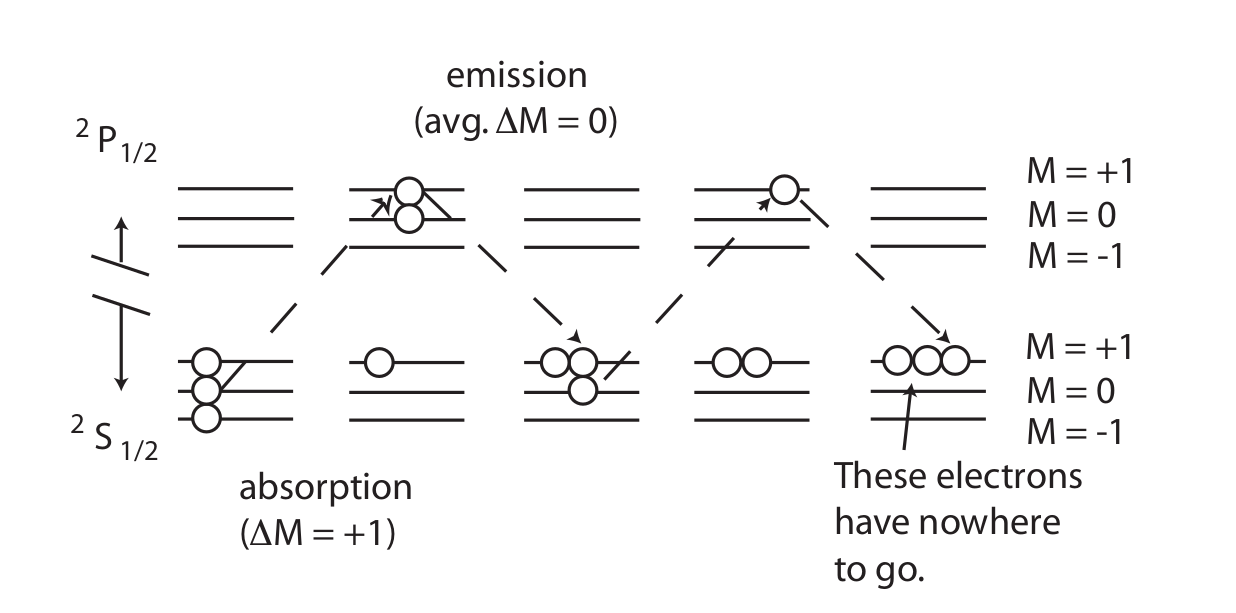
\includegraphics[width=0.8\textwidth]{content/img/optisches_pumpen.png}
    \caption{Schematische Darstellung des Prozesses \textit{optisches Pumpen} für Wasserstoff.
    Elektronen absorbieren zirkular polarisiertes Licht ($\Delta m = +1$) und 
    fallen über die spontane Emission wieder zurück in den Grundzustand ($\Delta m = 0, \pm 1$).
    Die Elektronen sammeln sich mit der Zeit im Grundzustand mit maximalen $m$ ($=+1$) an.
    }
    \label{fig:optisches_pumpen}
\end{figure}
Mit der Zeit sammeln sich die Elektronen im Grundzustand mit maximalen $m$ ($=1$) an.
Das Rubidiumgas ist polarisiert und die Photonen wechselwirken nicht weiter mit der Probe.
Oder anders anders ausgedrückt - die Probe ist jetzt transparent.
Dieser Zustand wird als Besetzungsinversion bezeichnet.
\\
\\
Bei dem Prozess des optischen Pumpens können Elektronen entweder über spontane Emission oder über induzierte Emission zurück in den Grundzustand fallen.
Induzierte Emission findet statt, wenn ein Photon die selbe Energie wie die Energiedifferenz der Zustände aufweist.
Das Photon induziert einen Übergang, wobei ein zweites Photon mit der selben Energie, Phase und Ausbreitungsrichtung emittiert wird.
\\
Spontane Emission stellt einen Spezialfall der induzierten Emission dar, die durch Vakuumsfluktuationen ausgelöst wird.
Die Wahrscheinlichkeit einer spontanen Emission ist proportional zu $~f^3$ und kann daher im Folgenden vernachlässigt werden.
\\
Die induzierte Emission kann durch ein angelegtes Hochfrequenzfeld (HF-Feld) erzeugt werden.
Dazu ist es notwendig, dass die durch das Feld deponierte Energie der Energiedifferenz des Übergangs entspricht.
Mit \autoref{eqn:zeeman_1} (der Energiedifferenz zwischen den Zeeman-Niveaus) folgt:
\begin{align}
    E_\text{HF} &= E_\text{Zeeman} \\
    \Rightarrow \:\:\: h f &= g_F \mu_B B_\text{res} \\
    \Rightarrow B_\text{res} &= \frac{4\pi m_e}{e g_F} f \label{eqn:resonanzfrequenz}
\end{align}
Wenn diese Bedingung erfüllt ist, findet induzierte Emission statt und die Besetzungsinversion wird aufgehoben.
Das Rubidiumgas verliert an Transparenz.

% Transiente Effekte?

\subsection{Magnetfeld einer Helmholtz-Spule}
Als Helmholtz-Spule werden zwei kreisförmige Spulen mit Radius $R$ bezeichnet, die im Abstand $R$ auf der gleichen Achse parallel aufgestellt sind.
Die Spulen besitzen jeweils $N$ Windungen und werden gleichsinnig von einem Strom $I$ durchflossen.
Zwischen den Spulen ergibt sich ein homogenes Magnetfeld.
\\
Aus dem Biot-Savart-Gesetz folgt für das Magnetfeld im Zentrum des Spulenpaars
\begin{equation}
    B = \frac{8}{\sqrt{125}} \frac{\mu_0 N I}{R} \, .
    \label{eqn:helmholtz}
\end{equation}